\documentclass[conference]{IEEEtran}

\usepackage[utf8]{inputenc}
\usepackage[T1]{fontenc}
\usepackage{amsmath}
\usepackage{graphicx}
\usepackage{booktabs}
\usepackage{array}
\usepackage{cite}
\usepackage{tikz}
\usepackage{pgfplots}
\usepackage[hidelinks]{hyperref}

\pgfplotsset{compat=1.18}
\usetikzlibrary{arrows.meta, positioning, shapes.geometric}

\title{Academic Collaboration Network: Simulation-Based Validation of a Skill Matching and Resource Sharing Platform}

\author{
\IEEEauthorblockN{Gabriel Andres Beltran Varela}
\IEEEauthorblockA{
Dept. of Computer Engineering\\
Universidad Distrital Francisco Jose de Caldas\\
Bogota, Colombia\\
gbeltranv@udistrital.edu.co}
\and
\IEEEauthorblockN{Kevin Santiago Silva Gonzalez}
\IEEEauthorblockA{
Dept. of Computer Engineering\\
Universidad Distrital Francisco Jose de Caldas\\
Bogota, Colombia\\
ksilvas@udistrital.edu.co}
\and
\IEEEauthorblockN{Miguel David Tarazona Correa}
\IEEEauthorblockA{
Dept. of Computer Engineering\\
Universidad Distrital Francisco Jose de Caldas\\
Bogota, Colombia\\
mtarazonac@udistrital.edu.co}
\and
\IEEEauthorblockN{Anyelo Esteban Casas Zapata}
\IEEEauthorblockA{
Dept. of Computer Engineering\\
Universidad Distrital Francisco Jose de Caldas\\
Bogota, Colombia\\
acasasz@udistrital.edu.co}
}

\begin{document}

\maketitle

\begin{abstract}
This paper presents the simulation and validation phase of the Academic Collaboration Network (ACN), a socio-technical platform designed to reduce isolated learning through skill-based group formation, collaborative workspaces, and institutional resource integration. The work consolidates the four-stage evolution of the project: system analysis, system design, robust project management, and computational validation. Primary survey data from Workshop 1 showed that 88\% of students relied exclusively on WhatsApp for academic coordination, 36\% identified lack of communication as the main barrier to group formation, and 96\% expressed positive or conditional interest in a dedicated collaboration platform. Building on the microservices architecture and risk-management strategy developed in Workshops 2 and 3, this study implements two complementary simulation approaches: a process-oriented discrete-event model and a behavior-oriented agent-based network model. Results show that the optimized ACN scenario reduces median group formation time by 91.5\%, improves satisfaction to 0.89, and maintains p95 matching latency at 1.24 seconds under a 500-student stress condition. The B1 isolation-priority loop reduces isolated students from 29 to 5 in the behavior model, validating the proposed design while identifying adoption as the main remaining implementation risk.
\end{abstract}

\begin{IEEEkeywords}
systems engineering, discrete-event simulation, agent-based modeling, collaborative learning, skill matching, social network analysis, academic platforms
\end{IEEEkeywords}

\section{Introduction}

Collaborative learning is widely recognized as an effective mechanism for improving academic performance, motivation, retention, and peer-supported knowledge construction \cite{johnson1998}. However, in many university environments, study groups are formed informally through personal contacts or messaging applications. This produces structural inefficiencies: skill clustering, isolated students, uneven access to academic support, and inefficient communication channels.

The Academic Collaboration Network (ACN) addresses this problem by treating study group formation as a systems engineering challenge. Students are modeled as nodes in a socio-technical network, while academic interactions represent edges through which knowledge and resources flow. From this perspective, isolated learning is not only an individual issue but also a network-structure problem: when collaboration depends on informal social proximity, high-connectivity students tend to accumulate more opportunities while peripheral students remain excluded \cite{wasserman1994,newman2010}.

Workshop 1 identified the main problem through primary data collection. A structured survey with $n=25$ students showed that 88\% relied exclusively on WhatsApp, 36\% reported lack of communication as the main barrier, and 96\% expressed positive or conditional interest in a platform for academic collaboration. Workshop 2 translated these findings into a microservices-based system design with a User Profile Service, Skill Matching Engine, Group Workspace, Notification Engine, Integration Gateway, and Analytics Dashboard. Workshop 3 strengthened the proposal through fault tolerance, risk management, quality assurance, a seven-month project plan, and a B1 balancing loop for isolation mitigation.

This fourth workshop completes the engineering cycle by validating the design through simulation. The central research question is: \emph{Does the proposed ACN architecture improve group formation efficiency, reduce isolated students, and remain feasible under stress and failure scenarios?} To answer this question, the paper implements process-oriented and behavior-oriented simulations calibrated with the previous workshops.

\section{Methods and Materials}

\subsection{System Evolution and Input Data}

The simulation is grounded in the project evolution summarized in Table~\ref{tab:evolution}. Workshop 1 contributes empirical parameters and the AS-IS baseline. Workshop 2 contributes architecture, functional requirements, and non-functional targets. Workshop 3 contributes risk scenarios, quality constraints, and the B1 feedback loop.

\begin{table}[htbp]
\caption{Project Evolution Across Workshops}
\label{tab:evolution}
\centering
\begin{tabular}{p{0.65cm} p{2.2cm} p{4.3cm}}
\toprule
\textbf{W} & \textbf{Primary Output} & \textbf{Contribution to Simulation} \\
\midrule
1 & System analysis & Survey data, AS-IS process, barriers, feedback loops \\
2 & System design & Microservices architecture, matching engine, latency targets \\
3 & Robust design & Risk register, QA gates, LMS fallback, B1 isolation loop \\
4 & Simulation & Empirical validation, scenarios, metrics, recommendations \\
\bottomrule
\end{tabular}
\end{table}

\subsection{Architecture Used for Simulation}

The ACN design follows a modular microservices architecture. Fig.~\ref{fig:architecture} summarizes the main components translated into simulation elements. Student profiles define skill, availability, performance, social connectivity, and platform openness. The Skill Matching Engine forms groups. Workspaces transform successful matches into collaboration edges. The Notification Engine affects invitation acceptance. The Integration Gateway improves schedule compatibility through LMS and library data. The Analytics Dashboard computes validation metrics.

\begin{figure}[htbp]
\centering
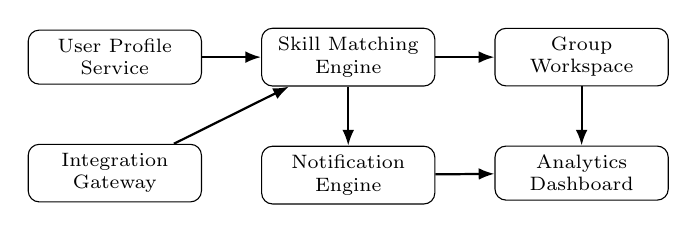
\begin{tikzpicture}[
node distance=0.75cm,
svc/.style={rectangle, draw, rounded corners, align=center, font=\scriptsize, minimum width=2.2cm, minimum height=0.65cm},
arr/.style={-{Latex[length=2mm]}, thick}
]
\node[svc] (profile) {User Profile\\Service};
\node[svc, right=of profile] (match) {Skill Matching\\Engine};
\node[svc, right=of match] (workspace) {Group\\Workspace};
\node[svc, below=of match] (notif) {Notification\\Engine};
\node[svc, below=of profile] (integration) {Integration\\Gateway};
\node[svc, below=of workspace] (analytics) {Analytics\\Dashboard};
\draw[arr] (profile) -- (match);
\draw[arr] (match) -- (workspace);
\draw[arr] (match) -- (notif);
\draw[arr] (integration) -- (match);
\draw[arr] (workspace) -- (analytics);
\draw[arr] (notif) -- (analytics);
\end{tikzpicture}
\caption{Simulated ACN architecture derived from Workshop 2.}
\label{fig:architecture}
\end{figure}

\subsection{Process-Oriented Simulation}

The first simulation is a process-oriented discrete-event model \cite{banks2010,law2015}. It represents the operational workflow from a student needing academic support to successful group formation. The AS-IS process uses informal social discovery and WhatsApp coordination, calibrated with the observed two-to-five-day formation window. Platform scenarios use automated matching, notification acceptance, schedule compatibility, and workspace activation.

The main process metrics are success rate, median formation time, p95 matching latency, isolated students, group balance index (GBI), and satisfaction. The Skill Matching Engine is evaluated against the Workshop 2 latency target of less than three seconds:

\begin{equation}
T(n)=\alpha n^2 + \beta n + \epsilon,
\end{equation}

where $n$ is the cohort size, $\alpha$ captures quadratic pairwise comparison growth, $\beta$ represents preprocessing overhead, and $\epsilon$ is stochastic runtime noise.

\subsection{Behavior-Oriented Simulation}

The second simulation is an agent-based network model \cite{railsback2019}. Students are agents and collaboration is represented as an undirected graph $G=(V,E)$. Weekly interactions create or reinforce edges. The model tracks density, isolated students, degree inequality, giant-component coverage, satisfaction, and adoption.

Network density is computed as:

\begin{equation}
Density=\frac{2|E|}{|V|(|V|-1)}.
\end{equation}

Degree centrality for a student $v_i$ is:

\begin{equation}
C_D(v_i)=\frac{deg(v_i)}{n-1}.
\end{equation}

The B1 balancing loop prioritizes students with low degree centrality, reducing the probability that isolated learners remain outside active collaboration groups.

\subsection{Scenario Design}

The simulation includes baseline, optimized, failure, and stress conditions, as requested by the workshop guide. Table~\ref{tab:scenarios} summarizes the scenarios.

\begin{table}[htbp]
\caption{Simulation Scenarios}
\label{tab:scenarios}
\centering
\begin{tabular}{p{1.8cm} p{3.0cm} p{2.2cm}}
\toprule
\textbf{Scenario} & \textbf{Purpose} & \textbf{Main Variation} \\
\midrule
AS-IS & Current informal coordination & No platform, homophily \\
ACN Baseline & Validate Workshop 2 design & 80\% adoption \\
Optimized B1 & Test isolation mitigation & B1 priority loop \\
LMS Outage & Validate fallback risk plan & LMS unavailable \\
Peak 500 & Stress test capacity target & 500 students \\
Low Adoption & Test adoption risk & 20\% initial adoption \\
\bottomrule
\end{tabular}
\end{table}

\subsection{Assumptions and Reproducibility}

The simulation uses synthetic profiles calibrated from the survey because real academic records are privacy-sensitive. Skill, availability, performance, social connectivity, and openness are normalized variables. The implementation is reproducible through a fixed random seed, but it also supports randomized seeds and custom CSV data to explore alternative cohorts.

\section{Results \& Discussion}

\subsection{Process Simulation Results}

Table~\ref{tab:process} presents the process-oriented simulation results. The optimized B1 scenario reduces group formation from 4.66 days in the AS-IS workflow to 0.40 days. It also improves satisfaction from 0.43 to 0.89 and reduces isolated students from 121.7 to 39.7 in the process model.

\begin{table}[htbp]
\caption{Process-Oriented Simulation Summary}
\label{tab:process}
\centering
\begin{tabular}{lrrrrr}
\toprule
\textbf{Scenario} & \textbf{Success} & \textbf{Days} & \textbf{p95(s)} & \textbf{Isolated} & \textbf{Sat.} \\
\midrule
AS-IS & 0.39 & 4.66 & N/A & 121.7 & 0.43 \\
Baseline & 0.91 & 0.38 & 0.27 & 68.8 & 0.87 \\
Optimized B1 & 0.98 & 0.40 & 0.21 & 39.7 & 0.89 \\
LMS Outage & 0.74 & 0.51 & 0.32 & 93.2 & 0.77 \\
Peak 500 & 0.94 & 0.39 & 1.24 & 130.0 & 0.87 \\
\bottomrule
\end{tabular}
\end{table}

\begin{figure}[htbp]
\centering
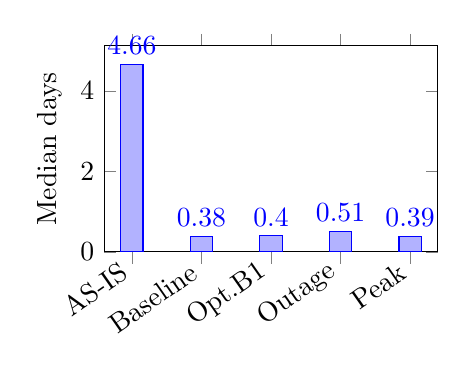
\begin{tikzpicture}
\begin{axis}[
ybar,
width=0.48\textwidth,
height=4.2cm,
ylabel={Median days},
symbolic x coords={AS-IS,Baseline,Opt.B1,Outage,Peak},
xtick=data,
x tick label style={rotate=35,anchor=east},
nodes near coords,
nodes near coords align={vertical},
ymin=0,
bar width=8pt
]
\addplot coordinates {(AS-IS,4.66) (Baseline,0.38) (Opt.B1,0.40) (Outage,0.51) (Peak,0.39)};
\end{axis}
\end{tikzpicture}
\caption{Median group formation time by scenario.}
\label{fig:formation}
\end{figure}

The stress scenario validates the feasibility of the matching engine. Even with 500 students, p95 latency remains at 1.24 seconds, below the three-second requirement defined in Workshop 2. The LMS outage scenario shows degradation but not collapse: success remains 0.74, confirming that the fallback strategy from Workshop 3 is necessary and effective.

\subsection{Behavior Simulation Results}

Table~\ref{tab:behavior} presents the behavior-oriented simulation results after 12 weeks. The AS-IS self-selection model ends with 29 isolated students and a density of 0.012. With B1 active, isolated students fall to 5, density rises to 0.116, and degree inequality decreases to 0.19.

\begin{table}[htbp]
\caption{Behavior-Oriented Simulation Summary}
\label{tab:behavior}
\centering
\begin{tabular}{lrrrrr}
\toprule
\textbf{Scenario} & \textbf{Adopt.} & \textbf{Density} & \textbf{Isolated} & \textbf{Gini} & \textbf{Sat.} \\
\midrule
AS-IS & 0.00 & 0.012 & 29 & 0.40 & 0.45 \\
No B1 & 0.51 & 0.026 & 7 & 0.43 & 0.63 \\
With B1 & 0.87 & 0.116 & 5 & 0.19 & 0.79 \\
Low Adoption & 0.37 & 0.026 & 11 & 0.47 & 0.62 \\
\bottomrule
\end{tabular}
\end{table}

These results validate the socio-technical logic of the design. The platform does not merely accelerate group formation; it changes the topology of the collaboration network. The B1 loop prevents isolated students from remaining peripheral by prioritizing low-degree nodes in group assignments.

\subsection{Validation of Design Decisions}

Table~\ref{tab:validation} maps simulation evidence to design decisions from previous workshops.

\begin{table}[htbp]
\caption{Design Validation Summary}
\label{tab:validation}
\centering
\begin{tabular}{p{2.2cm} p{3.4cm} p{1.2cm}}
\toprule
\textbf{Decision} & \textbf{Evidence} & \textbf{Result} \\
\midrule
Matching Engine & p95 latency 1.24s at 500 students & Validated \\
Workspace and notifications & Formation time reduced by 91.5\% & Validated \\
B1 isolation loop & Isolation reduced from 29 to 5 students & Validated \\
LMS fallback & Outage scenario remains operational & Partially validated \\
Adoption strategy & Low adoption leaves 11 isolated students & Needs mitigation \\
\bottomrule
\end{tabular}
\end{table}

\subsection{Complexity and Sensitivity Analysis}

The simulations reveal three complexity patterns. First, adoption produces nonlinear effects: once enough students participate, the graph becomes denser and matching quality improves. Second, informal self-selection concentrates centrality among already-connected students, increasing inequality. Third, the B1 balancing loop acts as a stabilizing mechanism by redistributing collaboration opportunities toward low-degree students.

The low-adoption scenario confirms that technical correctness is not sufficient. If adoption remains close to 20--40\%, isolated students persist even with a functioning matching engine. Therefore, the faculty ambassador strategy, guided onboarding, and early-access incentives proposed in Workshop 3 should be treated as technical risk controls, not as optional promotional activities.

\section{Conclusions}

This paper presented the simulation-based validation of the Academic Collaboration Network developed across the four workshops. The process-oriented simulation validated that the proposed platform can reduce group formation time, improve satisfaction, and remain below the three-second matching latency target under a 500-student stress scenario. The behavior-oriented simulation validated that the B1 isolation-priority loop reduces isolated students and improves network density and fairness.

Overall, the project successfully transforms an informal and socially biased group formation process into a structured, measurable, and optimizable socio-technical system. The main remaining challenge is adoption. Future work should include a real pilot with at least 50 students, replacement of synthetic profiles with consent-based institutional data, bias audits for the matching engine, and longitudinal validation across a full academic semester.

\section*{Acknowledgments}

The authors thank Eng. Carlos Andres Sierra, M.Sc., for guidance throughout the Systems Analysis \& Design course. The team also acknowledges the students who participated in the survey used to calibrate the Academic Collaboration Network.

\begin{thebibliography}{00}

\bibitem{johnson1998}
D. W. Johnson, R. T. Johnson, and K. A. Smith, ``Cooperative learning returns to college,'' \emph{Change}, vol. 30, no. 4, pp. 26--35, 1998.

\bibitem{wasserman1994}
S. Wasserman and K. Faust, \emph{Social Network Analysis: Methods and Applications}. Cambridge, U.K.: Cambridge University Press, 1994.

\bibitem{newman2010}
M. Newman, \emph{Networks: An Introduction}. Oxford, U.K.: Oxford University Press, 2010.

\bibitem{banks2010}
J. Banks, J. S. Carson, B. L. Nelson, and D. M. Nicol, \emph{Discrete-Event System Simulation}, 5th ed. Upper Saddle River, NJ, USA: Pearson, 2010.

\bibitem{law2015}
A. M. Law, \emph{Simulation Modeling and Analysis}, 5th ed. New York, NY, USA: McGraw-Hill, 2015.

\bibitem{railsback2019}
S. F. Railsback and V. Grimm, \emph{Agent-Based and Individual-Based Modeling}. Princeton, NJ, USA: Princeton University Press, 2019.

\bibitem{newman2021}
S. Newman, \emph{Building Microservices: Designing Fine-Grained Systems}, 2nd ed. Sebastopol, CA, USA: O'Reilly Media, 2021.

\bibitem{team2026w1}
Team 8, ``Workshop No. 1: Systems Analysis -- Academic Collaboration Network,'' Universidad Distrital Francisco Jose de Caldas, 2026.

\bibitem{team2026w2}
Team 8, ``Workshop No. 2: System Design -- Academic Collaboration Network,'' Universidad Distrital Francisco Jose de Caldas, 2026.

\bibitem{team2026w3}
Team 8, ``Workshop No. 3: Robust System Design and Project Management -- Academic Collaboration Network,'' Universidad Distrital Francisco Jose de Caldas, 2026.

\end{thebibliography}

\end{document}
